% !TEX TS-program = LuaLaTeX
\documentclass[10pt, oneside, a4paper]{article}

\usepackage[T1]{fontenc}
\usepackage{lmodern}
\usepackage{xcolor}
    \definecolor{gray} {HTML}{363636}
    \definecolor{red}  {HTML}{950009}
    \definecolor{green}{HTML}{0E610A}
    \definecolor{blue} {HTML}{020069}
\usepackage{fontspec}
    \setsansfont{Arial}
\usepackage{amsmath}
\usepackage{titlesec}
    \titleformat*{\section}      {\color{gray}\large\bfseries\sffamily}
    \titleformat*{\subsection}   {\color{gray}\large\bfseries\sffamily}
    \titleformat*{\subsubsection}{\color{gray}\large\bfseries\sffamily}
\usepackage{geometry}
    \geometry{scale={0.75,0.85}}
\usepackage{siunitx}
    \sisetup{locale=FR}
    \sisetup{math-micro=\text{µ},text-micro=µ} % fix
\usepackage{graphicx}
\usepackage{caption}
    \captionsetup{labelfont={bf,sf,color=gray}}
\usepackage{pdfpages}
\usepackage{caption}


% Keep lasts
\usepackage[french]{babel}
    \frenchsetup{SmallCapsFigTabCaptions=false}
\usepackage[expansion]{microtype}
\usepackage[luatex, backref]{hyperref}
    \hypersetup{unicode, colorlinks, breaklinks, urlcolor=red,
                bookmarksopen, bookmarksnumbered}

\renewcommand{\UrlFont}{\small}
\renewcommand{\arraystretch}{1.1}
\setlength{\parskip}{2mm}

\begin{document}

\begin{titlepage}
    \centering
    
\includegraphics[width=0.5\textwidth]{image/logo-ecam.png}\par
    \vspace{1cm}
    
    \rule{\linewidth}{1.5pt}%
    \vspace{5mm}
    {\rm\sffamily\LARGE Rapport de bureau d'étude\par}
    \vspace{3mm}
    {\sffamily\bfseries\LARGE Réalisation d'un amplificateur de classe D\par}
    \vspace{5mm}
    \rule{\linewidth}{1.5pt}%
    \vspace{1.5cm}
    
    {\Large%
        \begin{minipage}[t]{0.35\linewidth}
            \centering
            Alexis~\bsc{Nootens} \\[1mm]
            \href{mailto:16139@student.ecam.be}{16139@student.ecam.be}
        \end{minipage}
        \begin{minipage}[t]{0.35\linewidth}
            \centering
            Thomas~\bsc{Anizet} \\[1mm]
            \href{mailto:14164@student.ecam.be}{14164@student.ecam.be}
        \end{minipage}
    \par}
    \vfill
    
    {\large%
        ECAM Brussels             \\[1mm]
        Promenade de l'Alma 50    \\[1mm]
        1200 Woluwe-Saint-Lambert \\[1mm]
        Belgique
    \par}
    
    \vspace{2cm}
    {\large\today\par}
\end{titlepage}

%%%%%%%%%%%%%%%%
\tableofcontents
\newpage

%%%%%%%%%%%%%%%%%%%%%%%
\section{Introduction}
Après avoir étudié la théorie derrière le transfert de puissance en électronique,
nous avons mis à l'épreuve nos acquis théoriques dans un cas pratique en réalisant un circuit d'amplification de signaux audio analogiques.
Ce circuit d'amplification appartient à la classe D, une classe exploitant la connaissance de l'électronique de puissance, pour minimiser les pertes d'énergies aux étages d'amplification.
Ce document reprend notre réalisation et notre analyse du circuit.


%%%%%%%%%%%%%%%%%%%%%%%%%%%%%%%%
\section{Hypothèses de départ}
\label{sec:hypothese}
Avant de s'attaquer au problème, définissons l'environnement dans lequel nous allons travailler tel que la nature du signal reçu en entré.
Notre amplificateur doit être conçu pour les signaux audio ;
les signaux audio sont produit par un module convertisseur analogique-numérique (sigle CAN, ou DAC en anglais).
Leur tension est asymétrique entre \num{0} et une référence observée habituellement à \SI{1024}{\milli\volt} et leur fréquence varie entre \num{20} et \SI{22000}{\hertz}~\cite{heffner2007hearing}.
Nous supprimerons donc les composantes fréquentielles hors de ces bornes par des filtres passe-haut et passe-bas distincts.


%%%%%%%%%%%%%%%%%%%%%%%%%%%%%
\section{Circuit amplificateur}
Le circuit réalisé repose sur deux modules pour amplifier le signal d'entré :
un convertisseur analogique-numérique de type Sigma-Delta, et un contrôleur de transistor MOSFET.
La mise en série de ces deux modules permet de créer un amplificateur de classe D.
Les sous-sections \ref{sec:sigmaDelta} et \ref{sec:classeD} définissent le principe derrière chaque module et évoquent leur raison d'être.


\subsection{Modulation Sigma-Delta}
\label{sec:sigmaDelta}
Il existe une évolution des méthodes de modulation en pleine onde.
La plus simple est la modulation de largeur d'impulsion, MLI.
% Modulation de Largeur d'Impulsion
Voici comment elle fonctionne : depuis deux états possibles de tension, haut et bas, une période d'impulsion nommée \tau{}, et une durée variable de tension haute nommée $t$, le signal respecte la condition suivante : $0 \leq t \leq \tau $, soit $t \div \tau \in [0,1]$.
L'information modulée se situe dans le rapport de durée tension haute sur durée d'impulsion.
La donnée nécessite d'être transposée au préalable dans l'interval entre 0 et 1.
Cette modulation bénéficie de pouvoir être directement applicable comme commande d'un étage d'amplification en puissance.
Elle se traduit sans opération supplémentaire en commande complètement ouverte ou complètement fermée de transistor.

% Modulation Delta
Une évolution de la modulation de largeur d'impulsion est la modulation Delta.
Tandis que la MLI encode l'entièreté de l'information dans son rapport cyclique à chaque période, la modulation Delta n'encode que la différence (delta) par rapport à l'information précédente.
Les différences entre informations sont de taille plus petites que les informations entières.
Elles sont envoyées plus rapidement.
Ainsi, pour une période donnée, plus de delta pourront être envoyés que de cycles MLI complets.
Le modulateur fonctionnera à une fréquence plus élevée, suréchantillonnant le signal, ce qui réduit le bruit de quantification~\cite{gray1998quantization} par rapport à un modulateur MLI.

% Modulation Sigma-Delta
La modulation Delta connecte la sortie à l'entrée pour la différentier, c'est une rétro-action.
Un automaticien y reconnaîtra un contrôle en boucle fermée proportionnel, un régulateur P.
Cet automaticien saura également que ces régulateurs ont le défaut de toujours avoir un décalage entre la consigne et le signal de sortie désiré, nommé \og{}écart statique\fg{}.
Ce problème se résout en ajoutant un intégrateur avant la comparaison ; ce dernier maintient la dernière valeur comparu.
Cela devient un régulateur PI \og{}proportional-integral\fg{}.
Cette nouvelle modulation se nomme Sigma-Delta, puisqu'elle somme (\Sigma{}) les différences (\Delta{}).

Le schéma fonctionnel d'un circuit sigma-delta est présenté à la figure~\ref{fig:sigmaDelta}.
Voici son fonctionnement :
pour un signal d'entrée constant non nul, le différentiateur débute par soustraire le signal de sortie à l'entrée.
Si le système est reposé, la sortie est nulle et le signal d'entrée arrive pleinement à l'intégrateur.
L'intégrateur va introduire une temporisation dans le système ;
le signal à la sortie de l'intégrateur grimpe progressivement de manière monotone.
Ce signal arrive à l'entrée d'un comparateur qui retourne une tension soit maximale, soit minimale.
C'est ce signal binaire qui est réutilisé en rétro-action.
Le système va tenter de compenser le signal d'entrée avec la tension haute ou la tension basse.
Cette tension n'ayant pas de valeur intermédiaire, le système ne parviendra jamais à compenser le signal d'entré si celui-ci se trouve entre les bornes.
Le système est oscillant.
L'information modulée s'encode comme les différences entre cycle tension haute--basse.

\begin{figure}[htbp]
    \centering
    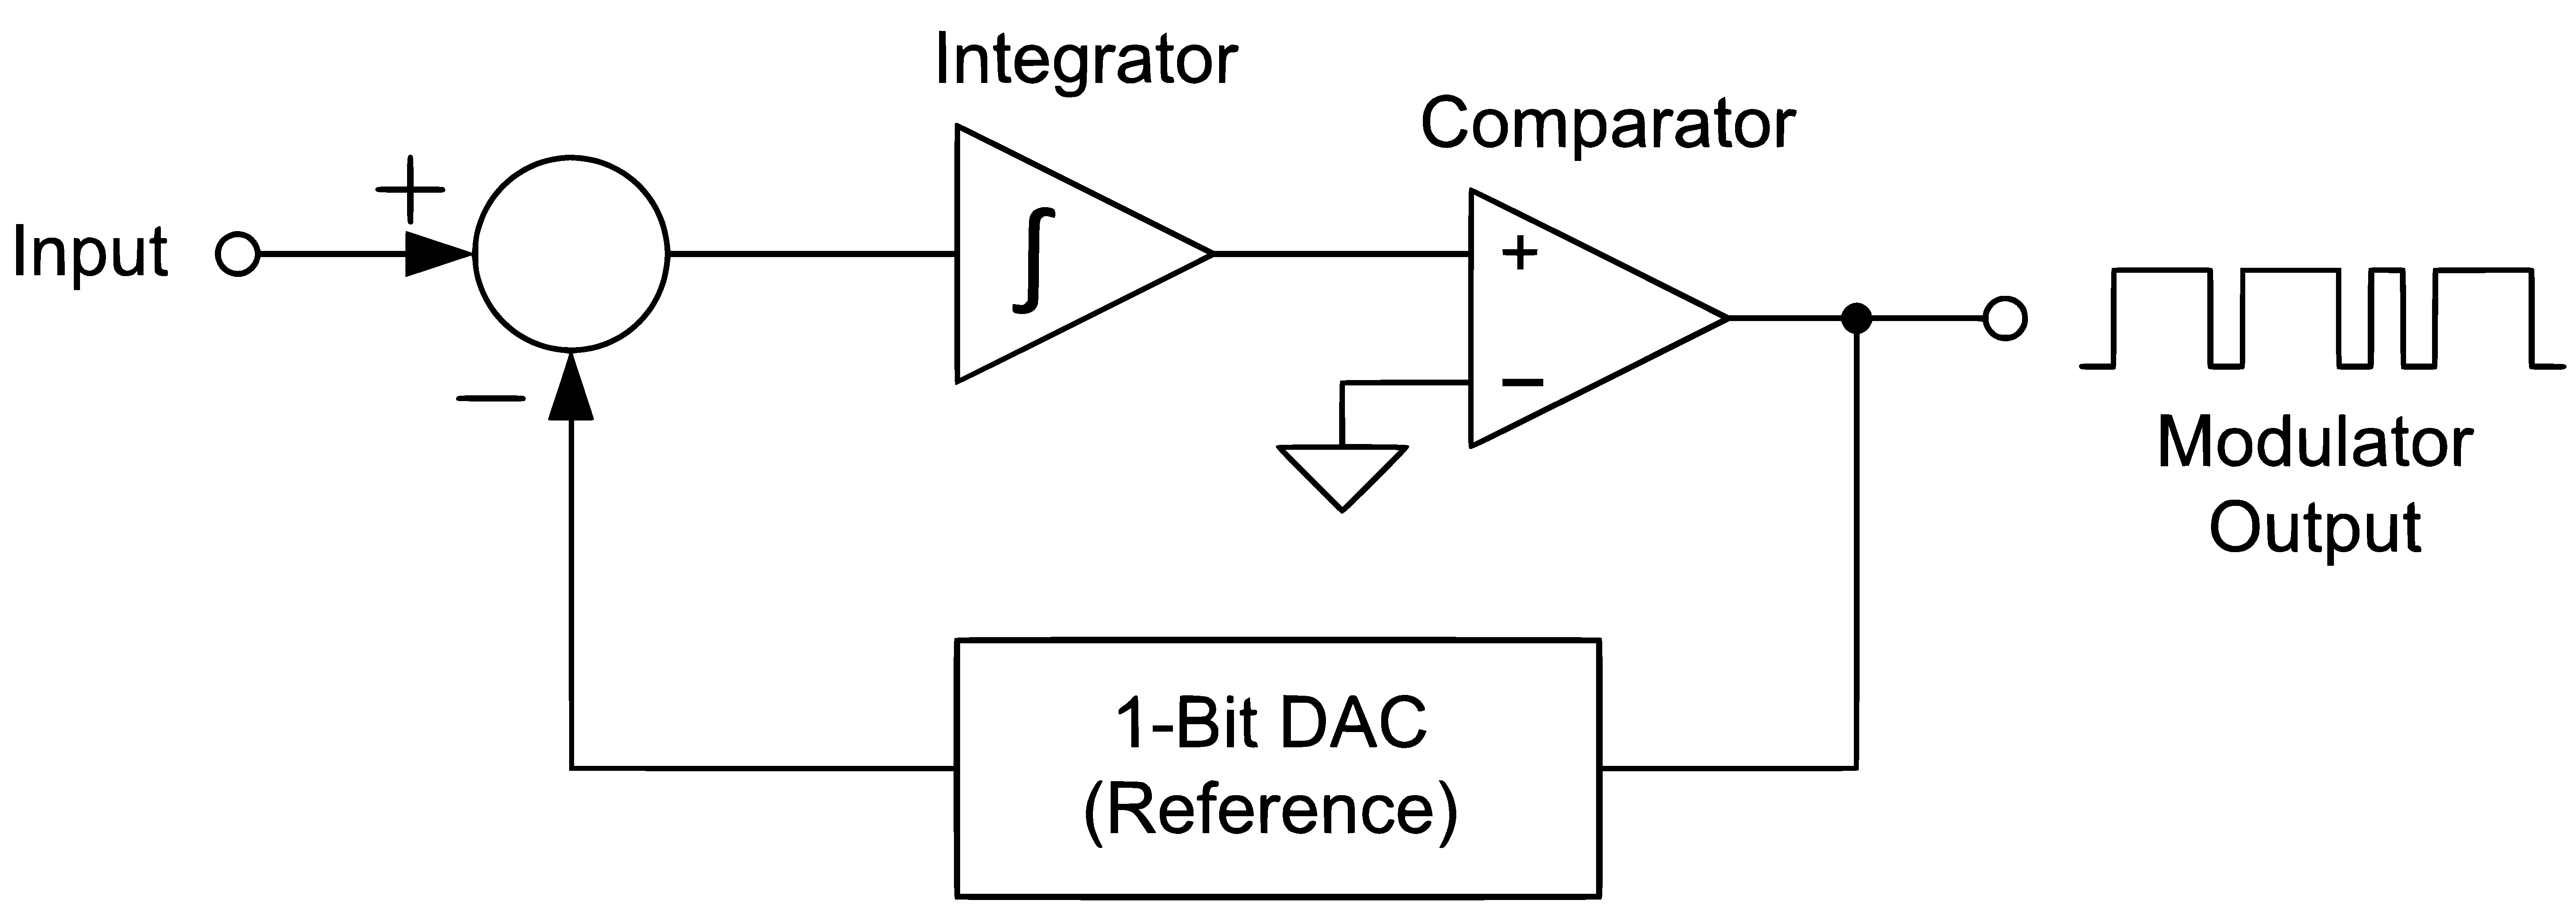
\includegraphics[width=0.7\textwidth]{eps/sigma-delta.eps}
    \caption{Schématique symbolique d'un modulateur \Sigma{}-\Delta{}.
    Le signal d'entrée \og{}Input\fg{} est de nature analogique.
    Le circuit agit en boucle fermée pour compenser la différence entre entrée et sortie.}
    \label{fig:sigmaDelta}
\end{figure}

\subsection{Amplificateur de classe D}
\label{sec:classeD}
La famille des amplificateurs contient plusieurs divisions --- dénommées \og{}classes\fg{} --- selon la nature du signal en sortie.
Par exemples :
les amplificateurs de classe A sortent une tension sinusoïdale amplifiée sur les deux crêtes ;
les amplificateurs de classe B ne laissent sortir qu'une seule crête amplifiée du sinus.

Les amplificateurs de classe D imposent des tensions aux rails d'alimentation du circuit.
C'est du tout ou rien.
Ils sont composés de transistor MOSFET.
Les transistors MOSFET sont les favoris de l'électronique de basse puissance.
Ils peuvent travailler à haute fréquence (plusieurs dizaines de kHz) et leur résistance à la conduction en saturation \og{}R\textsubscript{DS,ON}\fg{} est très faible (une centaine de m\Omega{} dans les basses puissances)~\cite{irf2017mosfet}.
Cette propriété donne tout son intérêt à l'amplificateur de classe D.
En ouvrant ou fermant complètement les transistors pour les faire fonctionner dans leur zone saturée, on minimise la résistance de conduction.
Sachant que la perte en conduction est dû à l'effet joule, et que la puissance de l'effet joule se formule comme $P=RI^2$~\cite{griffiths1999introduction}.
Lorsque $R$, la résistance du transistor est minimale, la puissance $P$ perdue à la conduction est minimisée pour une courant $I$ donné~\cite{sente2017elec}.
Le principe de l'amplificateur de classe D est présenté visuellement à la figure~\ref{fig:classeD}.
Un filtre LC peut-être placé à la suite de l'étage d'amplification pour lisser le courant et la tension~\cite{wildi2005electrotech}.
Dans notre réalisation, nous considérons que le bobinage du haut-parleur lissera le courant et nous ne placerons pas d'inductance discrète.

\begin{figure}[htbp]
    \centering
    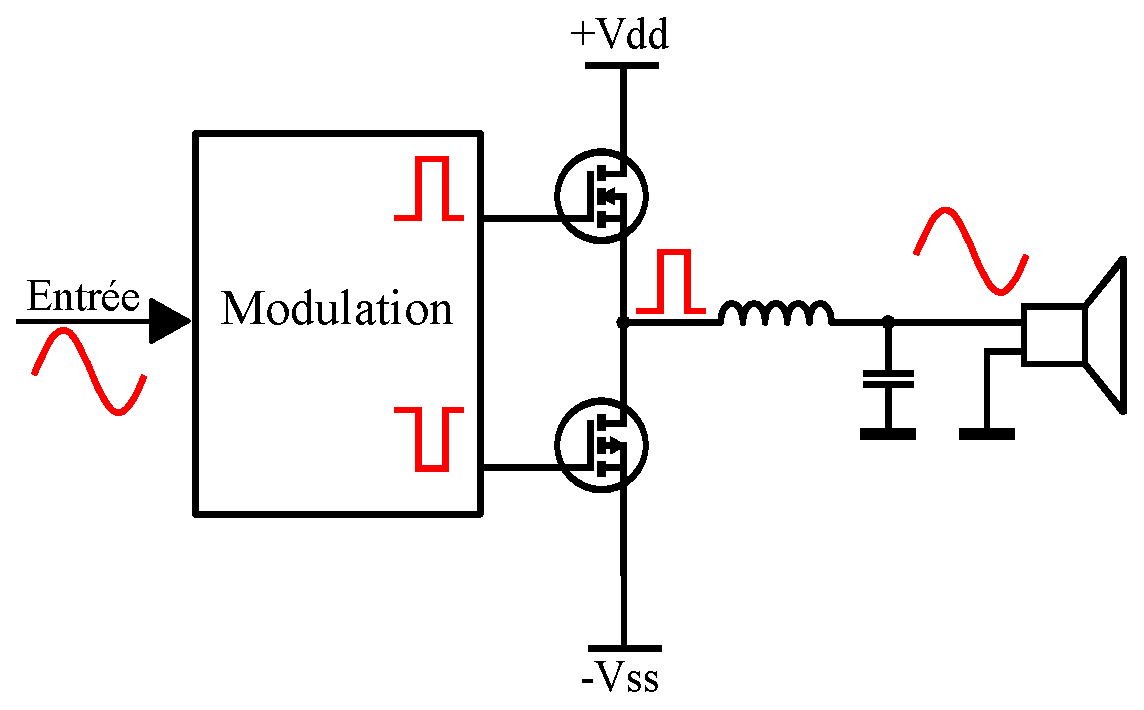
\includegraphics[width=0.5\textwidth]{eps/classe-d.eps}
    \caption{Schématique du principe de l'amplificateur de classe D.
             Le signal d'entré analogique est modulé en commande de commutation de
             transistor de puissance.
             Le signal amplifié se trouve à l'état $+\text{Vdd}$ ou $-\text{Vss}$
             uniquement.
             Ce signal est ensuite lissé au travers d'un filtre LC pour retrouver
             des tensions intermédiaires.}
    \label{fig:classeD}
\end{figure}


%%%%%%%%%%%%%%%%%%%%%%%%%%%%%%
\section{Filtrage des signaux}
À la section~\ref{sec:hypothese}, il a été considéré que la fréquence du signal d'entrée varie entre \num{20} et \SI{22000}{\hertz}.
Pour se débarasser des fréquences hors de cette bande, \textit{i.e.} du bruit, nous filtrons le signal.
Il existe 2 familles de filtre selon les composants électroniques utilisés :
\begin{itemize}
    \item\textbf{Les filtre passifs} sont réalisés avec des composants passifs uniquement : principalement des résistances, des inductances et des condensateurs.
        Leur gain ne peut dépasser 1.
    \item\textbf{Les filtres actifs} contiennent des composants actifs : des transistors et des amplificateurs opérationnels.
        Ils peuvent amener de la puissance et donc un gain supérieur à 1.
\end{itemize}
La réponse fréquentielle d'un filtre se définit comme l'évolution d'amplitude et de phase d'un signal le traversant en fonction de la fréquence.
Le diagramme de Bode est une représentation de la réponse fréquentielle.
Nous nous intéressons uniquement aux filtres passes-bas et passe-haut étant donné que ce sont les seuls utilisés dans le circuit.
\begin{itemize}
    \item\textbf{Les filtre passe-bas} laissent passer toutes les fréquences depuis
        la fréquence nulle jusqu'à la fréquence de coupure et atténue toutes les
        fréquences supérieures qui lui sont supérieures.
    \item\textbf{Les filtre passe-haut} atténuent toutes les fréquences depuis la
        fréquence nulle jusqu'à la fréquence de coupure et laisse passer toutes
        celles qui lui sont supérieures.
\end{itemize}
Pour rappel, la fréquence de coupure d'un filtre, notée par la suite $f_c$, est la fréquence limite de fonctionnement utile de ce filtre.
Elle est défini à \SI{-3}{\decibel}, là où le signal perd la moitié de sa puissance.
Ainsi, nous définissions deux fréquences de coupures :
\begin{itemize}
    \item la $f_c$ du filtre passe-bas à \SI{22000}{\hertz}
    \item la $f_c$ du filtre passe-haut à \SI{20}{\hertz}
\end{itemize}
La combinaison de ces deux filtres en série nous permettra d'obtenir une filtre passe-bande.


%%%%%%%%%%%%%%%%%%%%%%%%%%%%%%%%
\section{Schématique du circuit}
Depuis une vue d'ensemble, le circuit que nous avons réalisé peut se diviser en trois parties : les filtres d'entrées et de pré-amplification ; le comparateur Sigma-Delta, et l'étage de puissance.
Cette section présente successivement chacune de ces parties.
Les schémas complets sont disponibles aux annexes.

\subsection{Filtres d'entrées}
La figure~\ref{fig:schemaPreAmpli} présente les parties de pré-amplification et de filtrage reçues au cours.
Le trajet emprunté par le signal est le suivant : le signal analogique arrive sur la pin \texttt{ININV\underline{A}}.
La résistance \texttt{R15} n'existe pas.
Étant donné la nécessité d'un filtre passe-haut, un condensateur est ajouté entre les pins \texttt{ININV\underline{A}} et \texttt{ININV\underline{B}}.
C'est par là que le signal se dirige.
Une fois le condensateur traversé, le signal rencontre la résistance \texttt{R14} puis arrive à l'entrée inverseuse d'un amplificateur opérationnel avec rétro-action (\texttt{C18} et \texttt{R13}).
La sortie de cet AOP, dénommée par \texttt{OUTINV}, renvoie un signal filtré.

On peut apercevoir que le montage de filtrage et de pré-amplification n'est autre qu'une simple combinaison d'une implémentation élémentaire d'un filtre passe-haut et filtre passe-bas.
\begin{figure}[!ht]
    \centering
    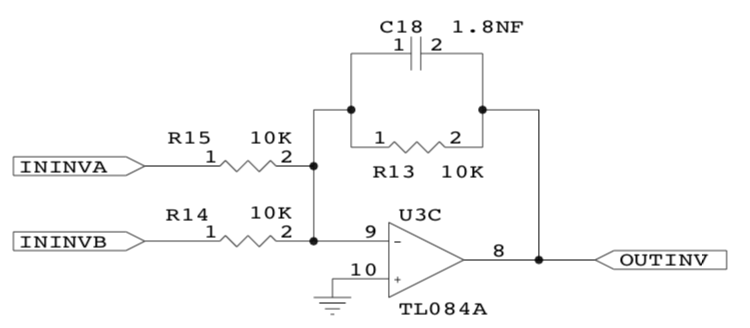
\includegraphics[width=0.6\textwidth]{image/schematique-all.jpg}
    \caption{Circuit schématique du filtre d'entrée et de préamplification de la partie
             Sigma-Delta.}
    \label{fig:schemaPreAmpli}
\end{figure}

Afin de mieux distinguer le montage, les figures~\ref{fig:filtreLowpass} et \ref{fig:filtreHighpass} présentent respectivement le circuit d'un filtre élémentaire passe-bas et d'un filtre passe-haut :

\begin{minipage}[t]{.45\textwidth}
    \centering
    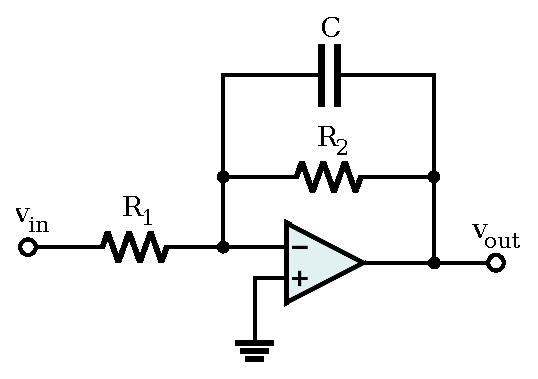
\includegraphics[height=110pt]{eps/active-lowpass-filter-rc.eps}
    \captionof{figure}{Implémentation élémentaire d'un filtre actif passe-bas déséquilibré.}
    \label{fig:filtreLowpass}
\end{minipage} \hfill
\begin{minipage}[t]{.45\textwidth}
    \centering
    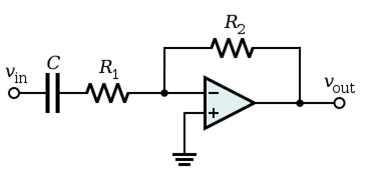
\includegraphics[width=\textwidth]{image/active-highpass-filter-rc.png}
    \captionof{figure}{Implémentation élémentaire d'un filtre actif passe-haut déséquilibré.}
    \label{fig:filtreHighpass}
\end{minipage}

\subsection{Alimentation}
La figure~\ref{fig:alimDecouplage} présente le circuit de découplage de l'alimentation.
Cela ne présente que peux d'intérêt mais est énoncé pour montrer son existence.

\begin{figure}[!ht]
	\centering
	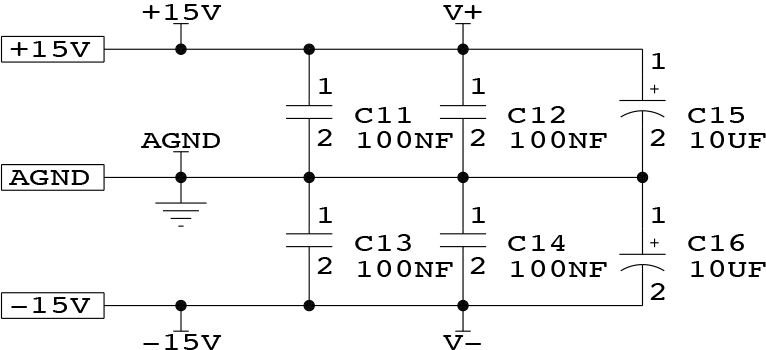
\includegraphics[width=6cm]{image/sch-alim.png}
	\caption{Schématique du circuit découplage d'alimentation.}
	\label{fig:alimDecouplage}
\end{figure}

\subsection{Comparateur Sigma-Delta}
La figure~\ref{fig:sch-ctrl} présente la partie logique du circuit, celle qui analyse le signal analogique et le module en commande d'ouverture de transistor.
Le signal rentre par la connection \texttt{OUTINV} provenant des filtres d'entrées de pré-amplifications.
À ce signal est ajouté la sortie actuelle du comparateur \texttt{VMLI} pour différentier l'erreur.
Comme la sortie du comparateur est bi-state en \SI{\pm15}{\volt}, si le signal à comparer est à \SI{0}{\volt}, la retro-action se placera à \SI{15}{\volt} et il y aura un décalage entre la valeur désiré et la valeur mesuré.
Pour adresser ce décalage, \SI{15}{\volt} sont directement retiré de la retro-action.

Le premier AOP \texttt{U3A} agit tel un intégrateur et intègre la différence entre la mesure et la consigne.
Le second AOP \texttt{U5B} réagit en trigger de Schmitt et fixe sa sortie en bi-state \SI{\pm15}{\volt} suivant que l'erreur entre la mesure et la consigne soit positive ou négative.

\begin{figure}[!ht]
	\centering
	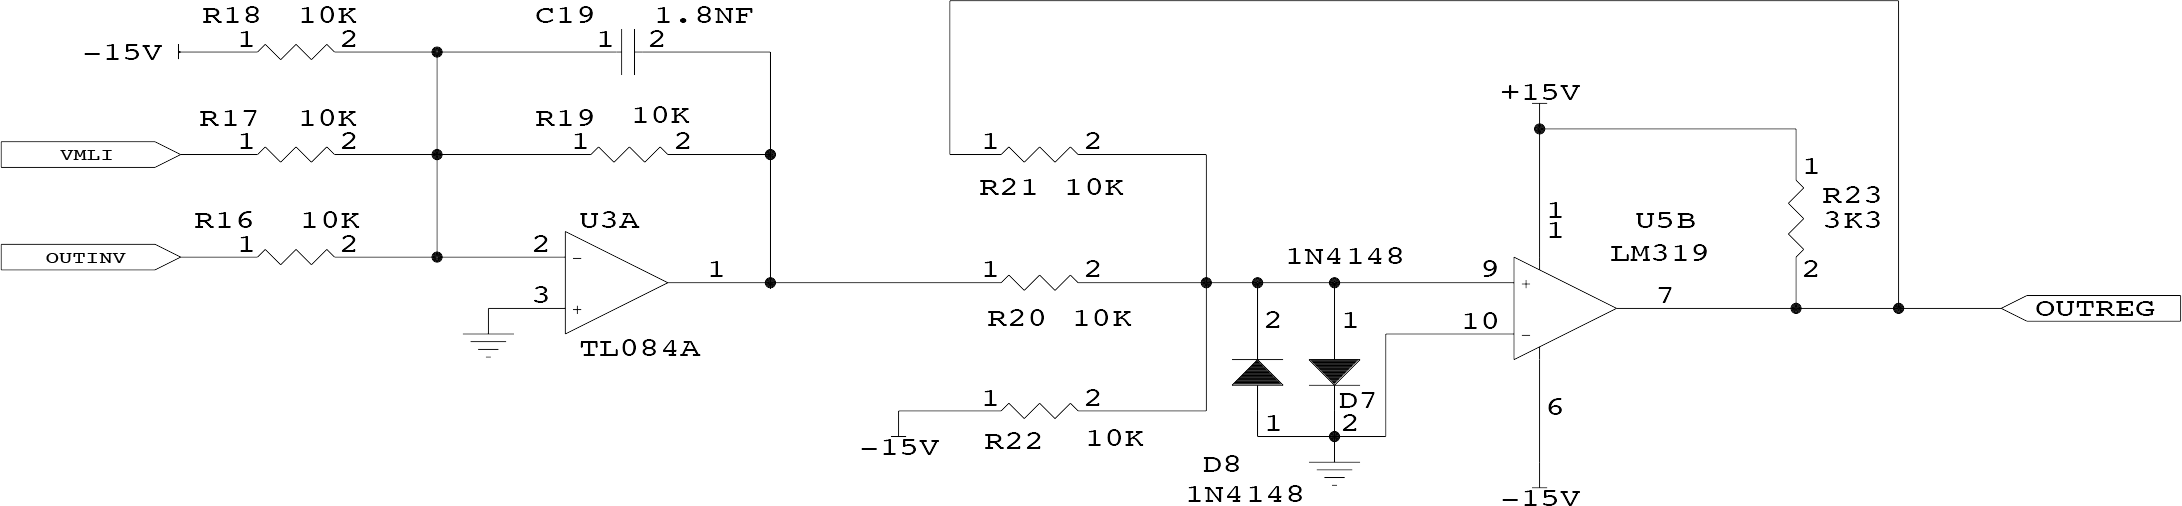
\includegraphics[width=\textwidth]{image/sch-ctrl.png}
	\caption{Schématique du circuit de comparaison Sigma-Delta.}
	\label{fig:sch-ctrl}
\end{figure}

\subsection{Étage de puissance}
La commande d'ouverture des transistors arrive par \texttt{CMDMOS}.
Ce signal est dédoublé dont l'une des sortie est inversée, afin de contrôler les deux transistors alternativement.
Le circuit intégré \texttt{L6385} se charge de commander les grilles des transistors en y plaçant une tension adaptée grâce à son condensateur de bootstrap.
Le haut-parleur, charge RL dans le circuit, est connecté à la junction entre le transistor MOS supérieur et l'inférieur au jumper 1.
Pour une raison de facilité, la source de tension \SI{24}{\volt} située au jumper 5 est relié à la même source que le driver MOS.

\begin{figure}[!ht]
	\centering
	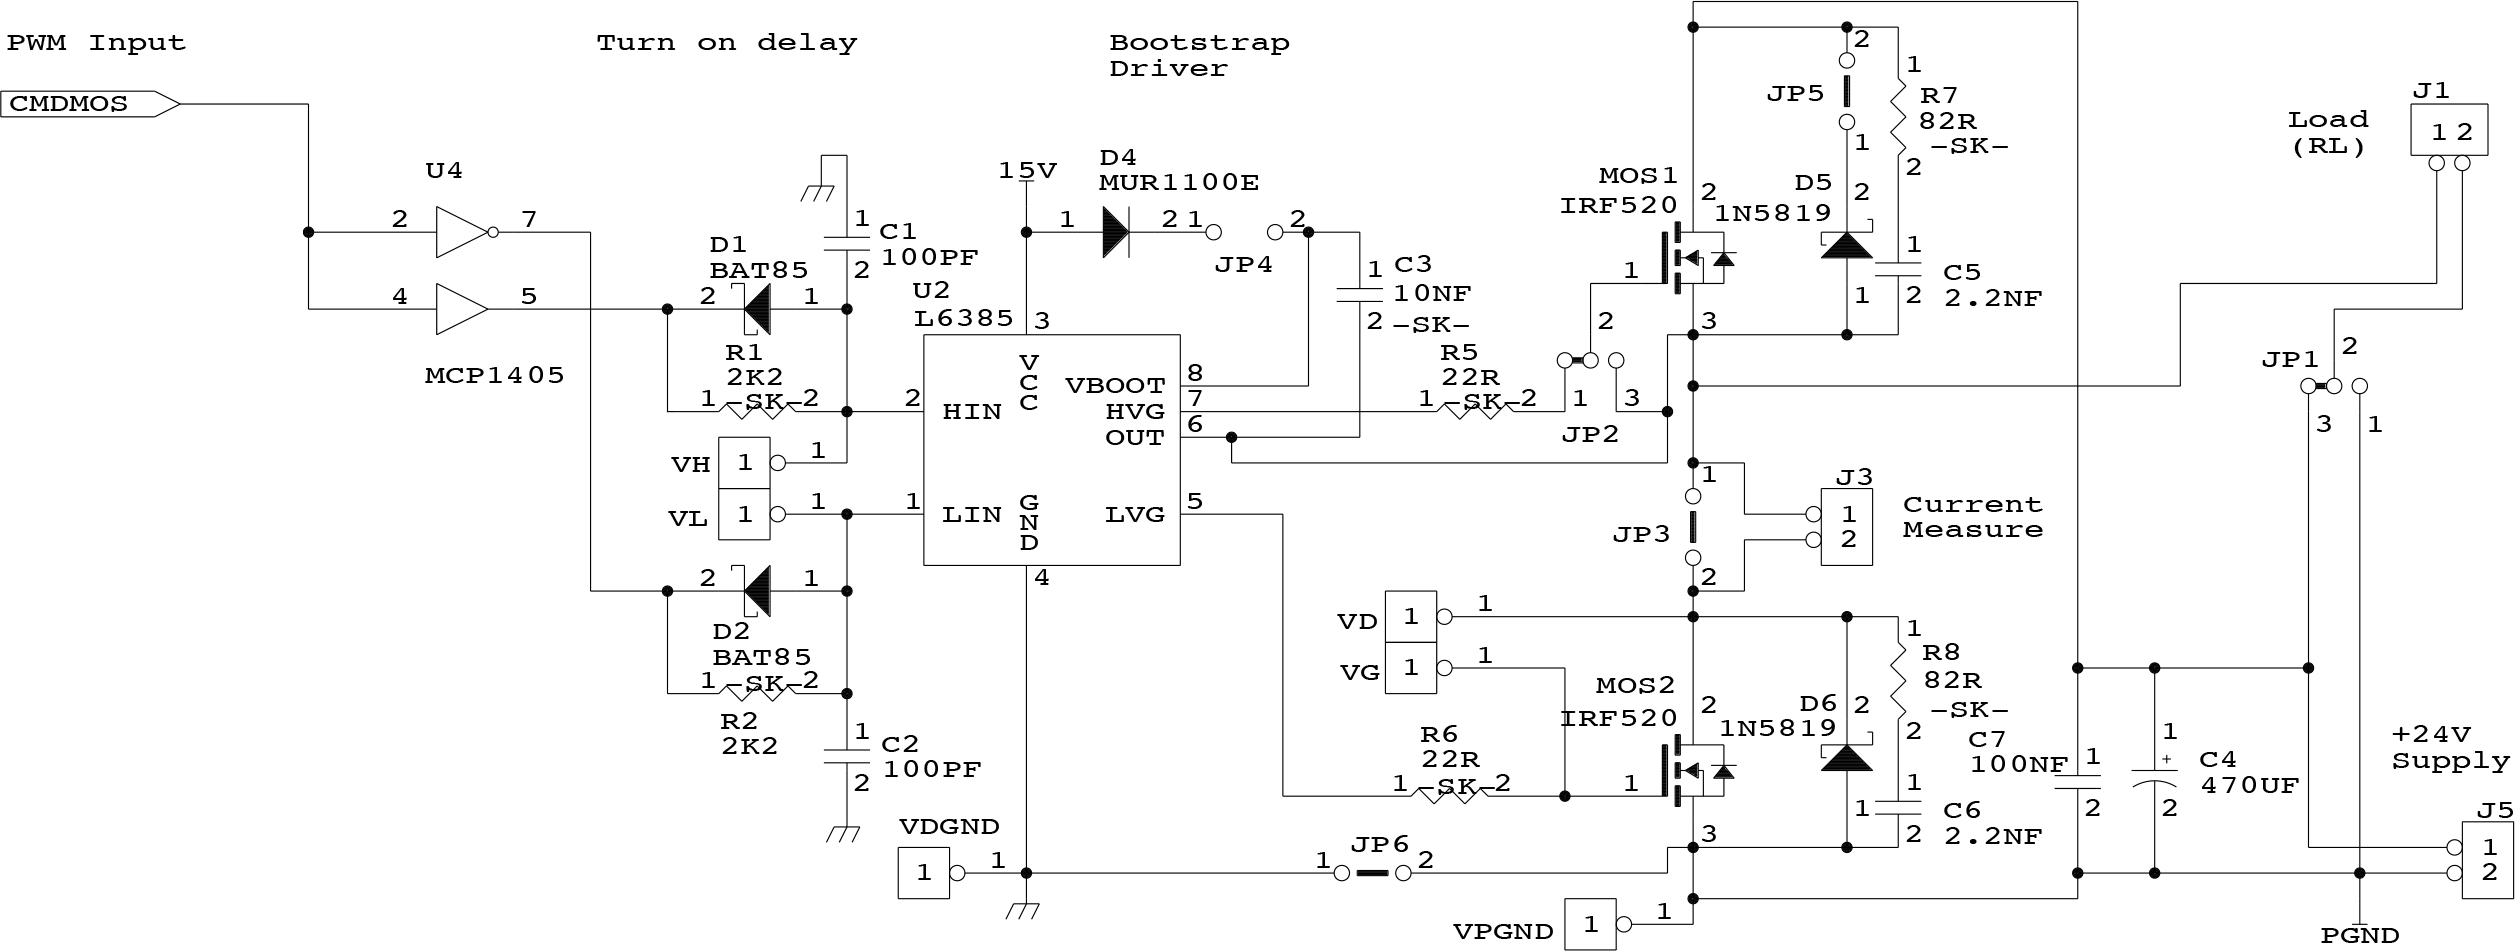
\includegraphics[width=\textwidth]{image/sch-mos.png}
	\caption{Schématique de l'étage de puissance, un circuit d'amplification par transistor
			 MOS.}
	\label{fig:sch-mos}
\end{figure}

%%%%%%%%%%%%%%%%%%%%%%%%%
\section{Dimensionnement}
Cette section aborde nos choix de composant dans la réalisation des filtres et du temps d'intégration du Sigma-Delta.
Ces choix sont accompagnés de calcules appuyant nos décisions.

\subsection{Filtres d'entrées}
\label{sec:filtrePreAmpli}
Pour dimensionner les composants électroniques (résistances et condensateurs) des deux filtres de l'amplificateur classe D, nous avons procédé comme suit :

\textit{N.B.} : Se référer aux figures~\ref{fig:filtreLowpass} et \ref{fig:filtreHighpass} pour les notations.
Les éléments R1 et C1 sont connectés entre l'entrée et la borne négative de l'AOP, les éléments R2 et C2 sont connectés à la rétro-action de cet AOP.

\noindent\textbf{Pour le filtre passe-bas} : durant le laboratoire, nous avons commencé par
dimensionner le filtre passe-bas.
La fréquence de coupure doit se trouver aux environ de \SI{20}{\kilo\hertz}.
Prendre les formules théoriques permettant de calculer la fréquence de coupure
et le gain de l'amplificateur :
\begin{gather}
    f_c = \frac{1}{2\pi R_2 C_2} \\
    A_v = -\frac{R_2}{R_1}
    \intertext{Poser comme hypothèse que nous souhaitons un gain unitaire.
			   Cela signifie que la valeur de la résistance R1 est égale à la valeur
			   de la résistance R2.}
    A_v = - \frac{R_2}{R_1} = -1
	\intertext{Fixer une valeur standard pour R2 et réécrire la formule permettant
			   de trouver la valeur de C2.
			   Nous avons pris une valeur standard de \SI{8.2}{\kilo\Omega} pour la résistance R2.}
    R_1 = R_2 = \SI{8.2}{\kilo\Omega} \\
    C_2 = \frac{1}{2\pi R_2 f_c}
    \intertext{Cherchant une valeur la plus standardisée possible pour le condensateur
    		   C2, nous devons ajuster la valeur de la fréquence de coupure dans la
		   	   formule donnée précédemment.
			   Ceci nous conduit à ajuster la fréquence de coupure à \SI{19400}{\hertz}.}
    C_2 = \frac{1}{2\pi\;8200\times19400} = \SI{1}{\nano\farad}
\end{gather}

\noindent\textbf{Pour le filtre passe-haut} : la fréquence de coupure doit se trouver aux environ
de 20 Hz.
Nous connaissons déjà les valeurs standards des deux résistances R1 et R2 ainsi que
du condensateur C2.
Il nous reste donc à calculer la valeur standard du condensateur C1.
Prendre la formule théorique permettant de calculer la fréquence de coupure
\begin{gather}
    f_c = \frac{1}{2\pi R_2 C_1}
	\intertext{Réécrire la formule permettant de calculer la valeur standard de C1}
    C_1 = \frac{1}{2\pi R_2 f_c}
	\intertext{Connaissant la valeur de R2, nous trouvons la valeur de C1 en ajustant
			   la valeur de la fréquence de coupure. Nous trouvons finalement une
			   fréquence de coupure de 18 Hz.}
    C_1 = \frac{1}{2\pi R_2 f_c} = \frac{1}{2\pi\,8200\times18} = \SI{1}{\micro\farad}
\end{gather}
Le tableau~\ref{tab:recapFiltres} reprend les valeurs calculées pour les filtres passe-bas et passe-haut :
\begin{table}[htbp]
    \centering
    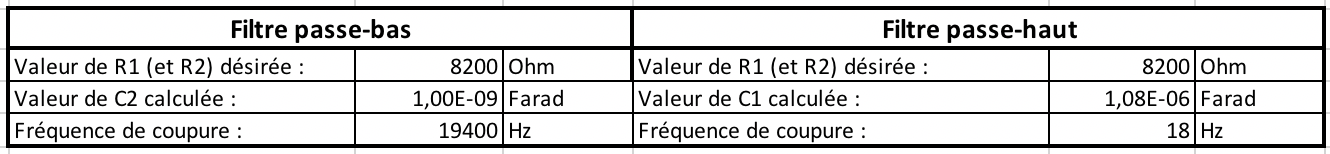
\includegraphics[scale=0.65]{image/tableau-filtres.jpg}
    \caption{Tableau récapitulatif des valeurs calculées pour les filtres de l'amplificateur classe D.}
    \label{tab:recapFiltres}
\end{table}

\subsection{Constante de temps du Sigma-Delta}
% TODO

\subsection{Filtre RC de sortie}
% TODO

%%%%%%%%%%%%%%%%%%%%%%%%%%%%
\section{Analyse du circuit}
Après que les éléments aient été dimensionnée, nous avons opté pour analyser le circuit en le faisant fonctionner en régime normal et en prenant des mesures en différents points.
Ces mesures sont toujours, sauf si cité explicitement, en tension par rapport à la masse, elle même mise à la terre.

\subsection{Défaut de fabrication}
Dés le premier branchement de la carte en tension symétrique \pm\SI{25}{\volt}DC,
nous avons observé un appel de courant de \SI{200}{\milli\ampere} sur le circuit.
Cette valeur était le maximum parametré sur l'alimentation de laboratoire à notre portée.
Ce courant est trop élevé pour un amplificateur au repos, c.-à-d. sans signal d'entrée.
Il n'y a nul doute qu'un problème de connexion existe sur la carte.

Pour cerner le problème, nous avons connecté un ohmmètre entre les bornes d'alimentation : positive-négative, positive-neutre, neutre-négative.
À ces bornes nous avons mesuré respectivement une résistance de : \SI{33}{\Omega}, \SI{9}{\kilo\Omega} et \SI{9}{\kilo\Omega}.
C'est désormais déterminé et mesuré, il existe un défaut de connexion entre la borne positive et le neutre.

Une analyse bloc-par-bloc a permis de déterminer que le problème était le circuit intégré \texttt{TC4428}, un double inverseur présentant un courant de fuite de \SI{100}{\milli\ampere} pour une tension d'alimentation de seulement \SI{4.3}{\volt};
ce qui est déraisonnable et en opposition avec la fiche technique du produit.
Nous en avons déduit que le composant était détruit.

Après avoir remplacé le circuit intégré \texttt{TC4428}, nous avons observé que la résistance entre la borne d'alimentation positive et le neutre passait de \SI{33}{\Omega} à \SI{200}{\Omega}, ce qui n'est toujours pas acceptable.
Nous avons remplacé un second circuit intégré douteux, le \verb|L6385E|, et la résistance est passée de \SI{200}{\Omega} à \SI{19}{\kilo\Omega}; ce qui est désormais raisonnable.
Tout cela démontre que deux des circuits imprimés ont été détruits.
Nous ne savons pas déterminer l'instant auquel cela s'est produit.

\subsection{Filtres d'entrées}
Voulant savoir si les valeurs théoriques calculées au point~\ref{sec:filtrePreAmpli}
conduisent à des filtres de fidèle qualité, nous les avons testé.
Nous avons donc tracé, dans le diagramme de Bode de chaque filtre.
Pour ce faire, nous avons utilisé :
\begin{enumerate}
    \item\textbf{Un générateur de signaux} pour générer un signal analogique
        d'amplitude et fréquence connue.
        L'objectif est de faire varier la fréquence du signal d'entrée et d'observer les
        conséquences que cela a sur l'amplitude du signal de sortie.
    \item\textbf{Un oscilloscope} pour mesurer les amplitudes des signaux à l'entrée du
        filtre et à la sortie de ce dernier.
\end{enumerate}

Les tables~\ref{tab:gainFiltresEntrees} reprennent les valeurs mesurées à l'oscilloscope, à savoir tension d'entrée et tension de sortie, ainsi que le calcul du gain en décibel pour chacun des deux filtres :
\begin{table}[!ht]
    \centering
    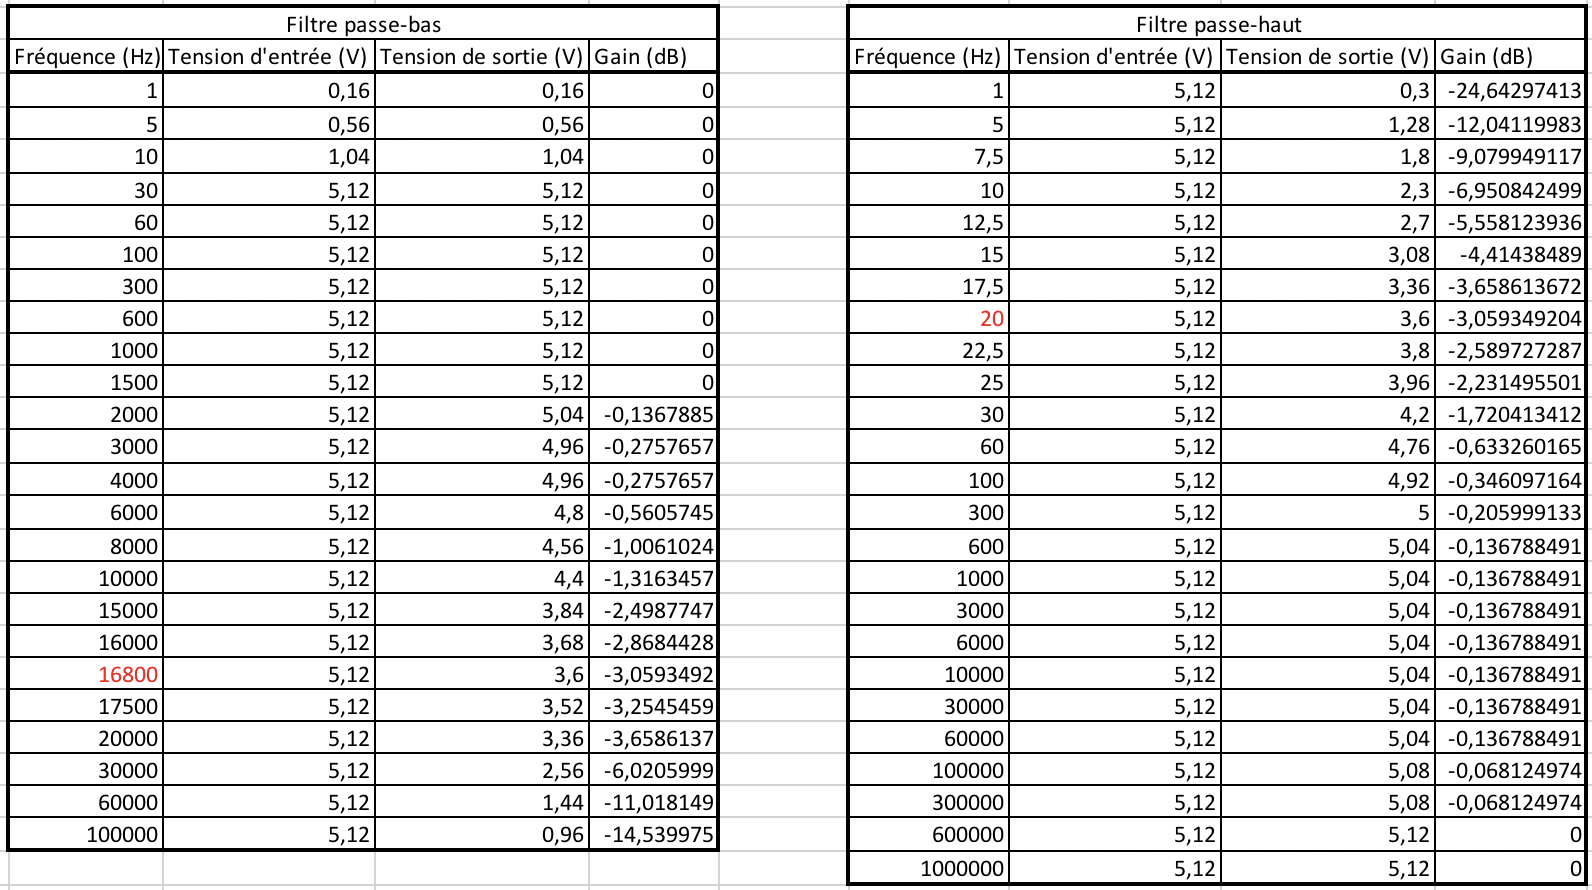
\includegraphics[scale=0.57]{image/resultat-filtres.jpg}
    \caption{Récapitulatif des valeurs mesurées pour les filtres d'entrées.}
    \label{tab:gainFiltresEntrees}
\end{table}

Nous avons réalisé un script Matlab\textregistered{} reprenant toutes les valeurs mesurées et reprises aux tables~\ref{tab:gainFiltresEntrees} afin de représenter la réponse fréquentielle de chacun des filtres dans le diagramme de Bode.
La figure~\ref{fig:resultatRepFreq} présente le résultat obtenu.
Nous pouvons y reconnaitre au gain qu'il s'agit de filtres Butterworth d'ordre 1~\cite{Horowitz:2015aa}.
\begin{figure}[!ht]
    \centering
    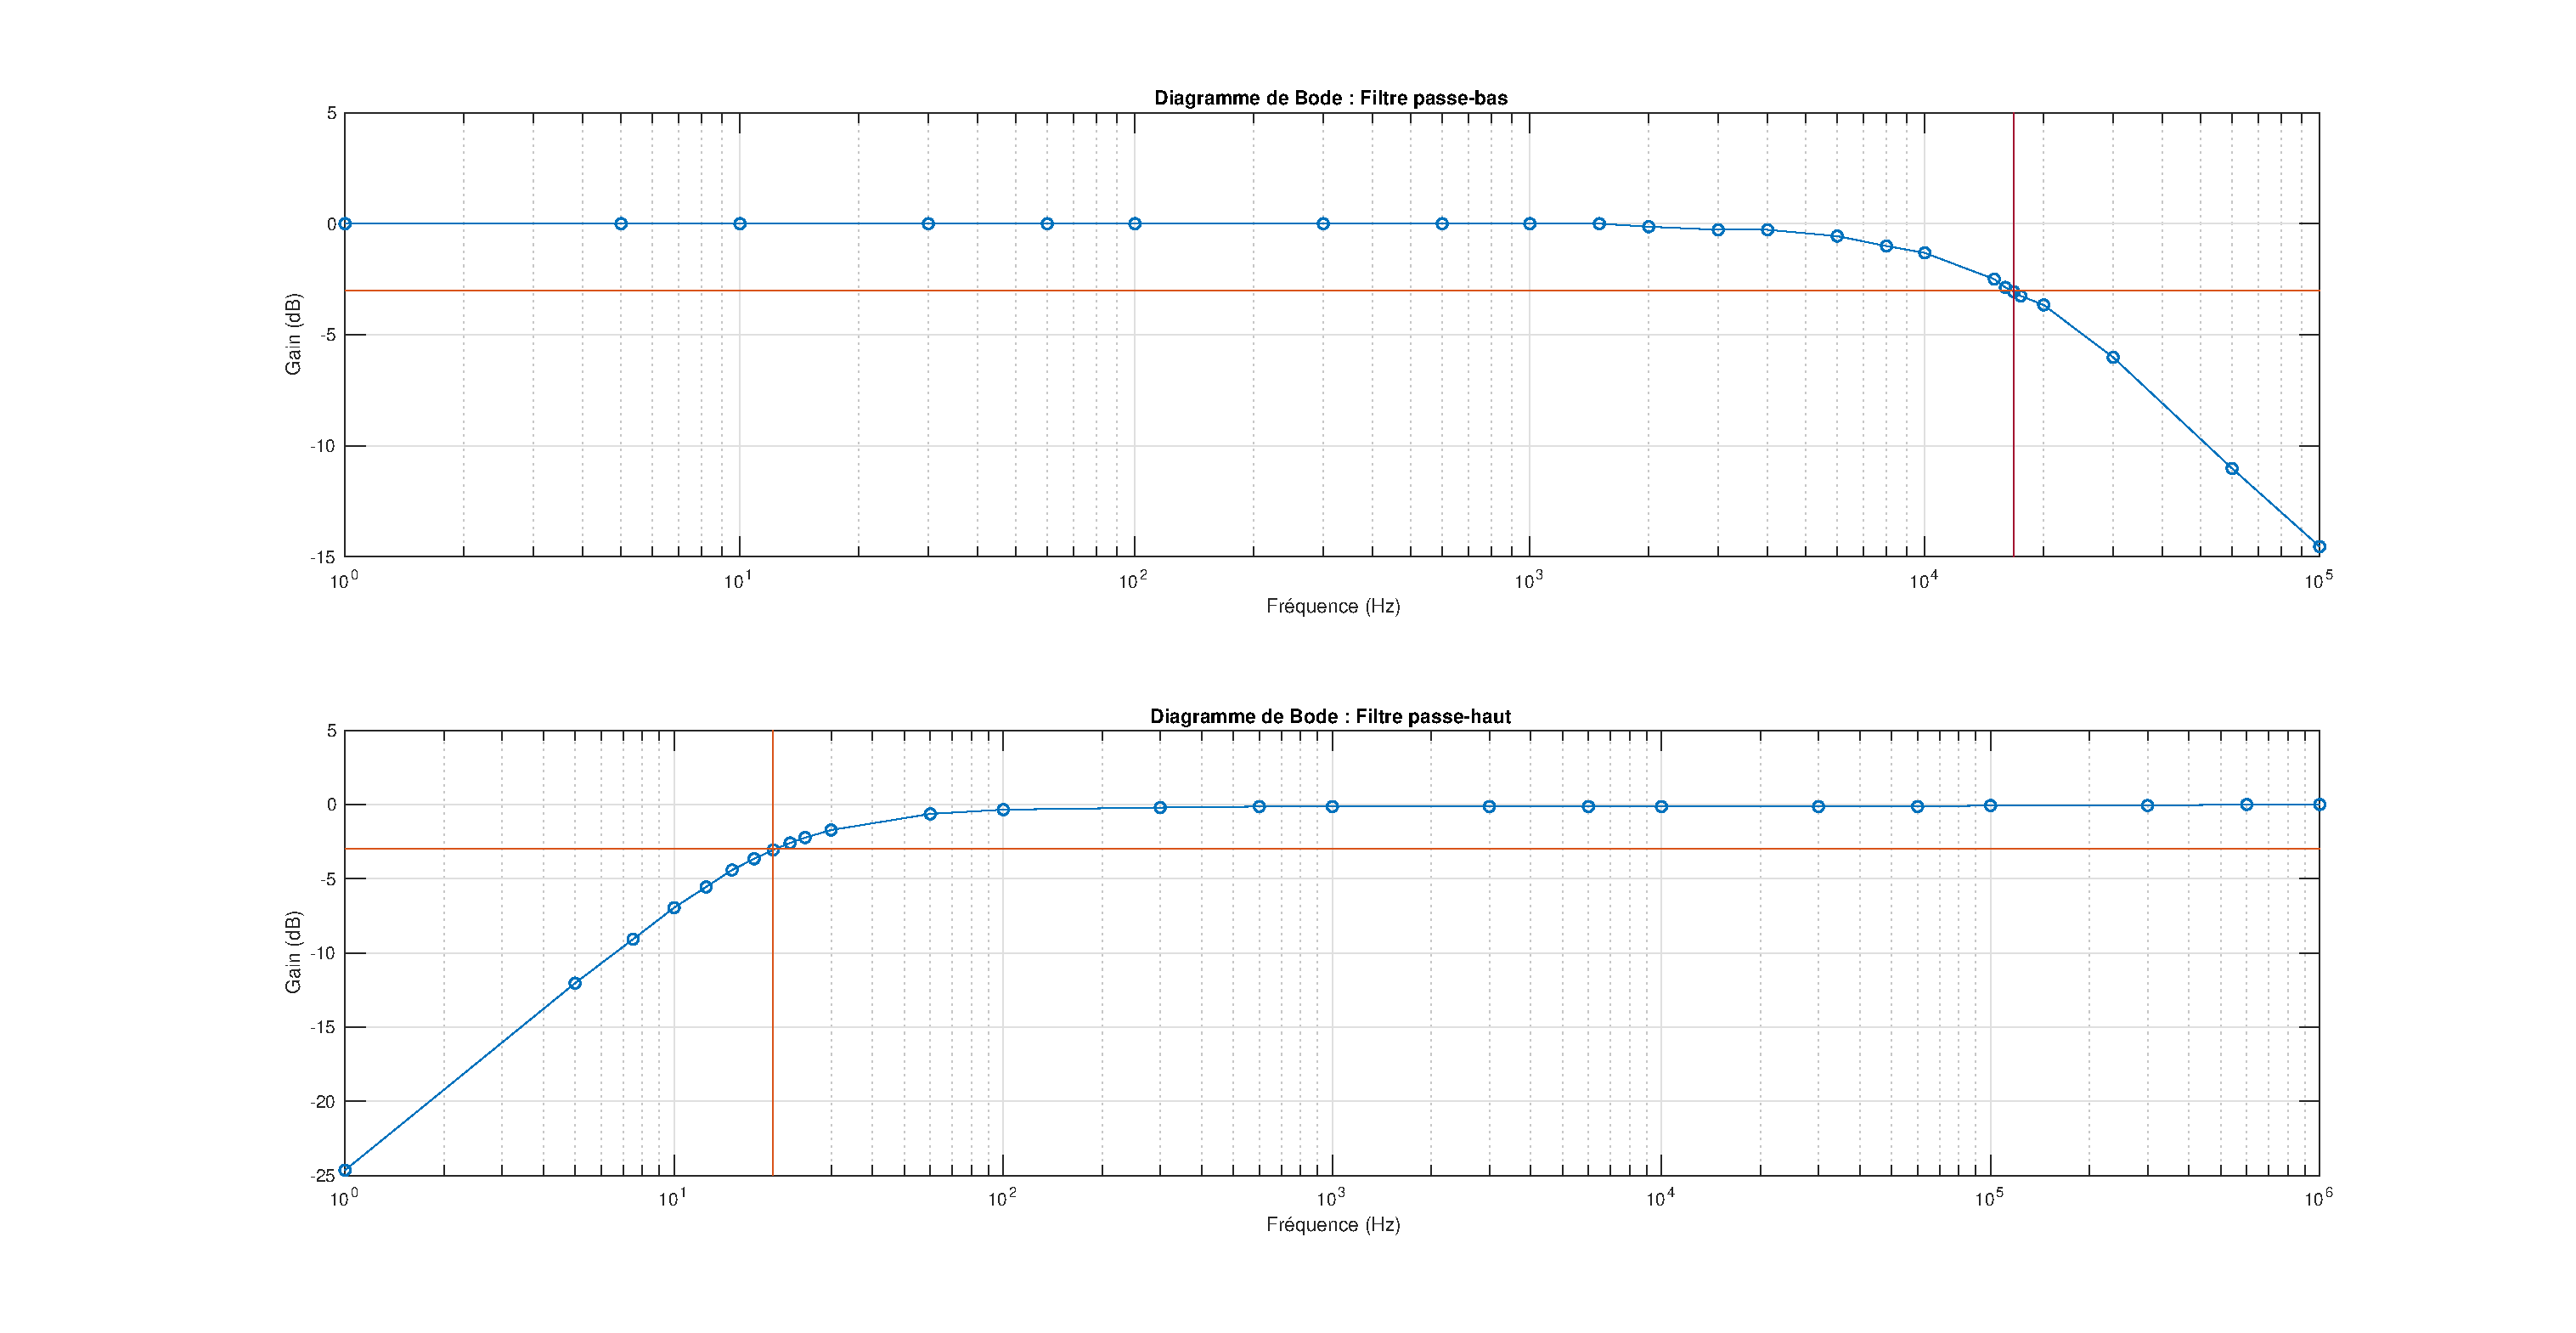
\includegraphics[width=\textwidth]{eps/bode-filtres.eps}
    \caption{Réponse fréquentielle pour les filtres passe-bas
             et passe-haut de l'amplificateur classe D.}
    \label{fig:resultatRepFreq}
\end{figure}

\subsection{Amplification}

\begin{figure}[!ht]
	\centering
	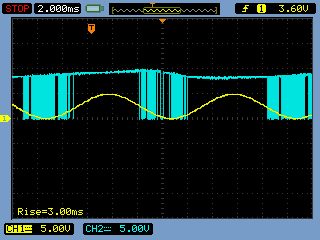
\includegraphics[width=0.65\textwidth]{image/osci-cmdmos.png}
	\caption{}
	\label{fig:}
\end{figure}

\begin{figure}[!ht]
	\centering
	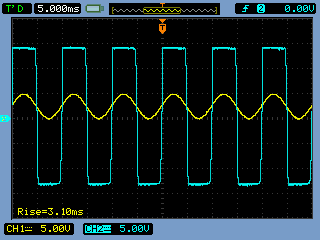
\includegraphics[width=0.65\textwidth]{image/osci-compar.png}
	\caption{}
	\label{fig:}
\end{figure}

\begin{figure}[!ht]
	\centering
	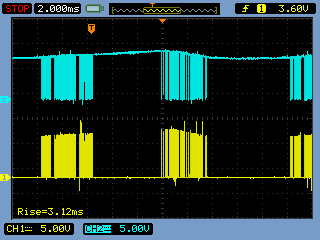
\includegraphics[width=0.65\textwidth]{image/osci-high-low.png}
	\caption{}
	\label{fig:}
\end{figure}

\begin{figure}[!ht]
	\centering
	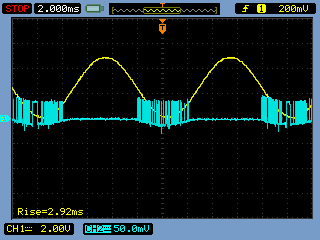
\includegraphics[width=0.65\textwidth]{image/osci-speaker.png}
	\caption{}
	\label{fig:}
\end{figure}

%%%%%%%%%%%%%%%%%%%%%
\section{Conclusion}


%%%%%%%%%%%%%%%%%%
\section*{Crédits}
\pdfbookmark[1]{Crédits}{sec:credits}
    
\begin{itemize}
\item Figure~\ref{fig:sigmaDelta} provenant de :\\*
Le blog officiel de Texas Instrument :
\url{https://e2e.ti.com/blogs_/archives/b/precisionhub/archive/2015/01/21/delta-sigma-adc-basics-understanding-the-delta-sigma-modulator}

\item Figure~\ref{fig:classeD} provenant de :\\*
Par Yves-Laurent (Travail personnel) [GFDL (\url{http://www.gnu.org/copyleft/fdl.html}),
CC-BY-SA-3.0 (\url{http://creativecommons.org/licenses/by-sa/3.0/})], de Wikimedia Commons

\item Figure~\ref{fig:filtreLowpass} provenant de :\\*
Par Inductiveload (Travail personnel) [Public domain], de Wikimedia Commons

\item Figure~\ref{fig:filtreHighpass} provenant de :\\*
Par Toriicelli (Travail personnel) [Public domain], de Wikimedia Commons
\end{itemize}

%%%%%%%%%%%%%%%%%%%%%%%%%%%%%%%%%%%%%%%%%%%
\pdfbookmark[1]{Références}{sec:references}
\bibliographystyle{unsrt}
\bibliography{ampli-classe-d}

%%%%%%%%%
\appendix
\clearpage
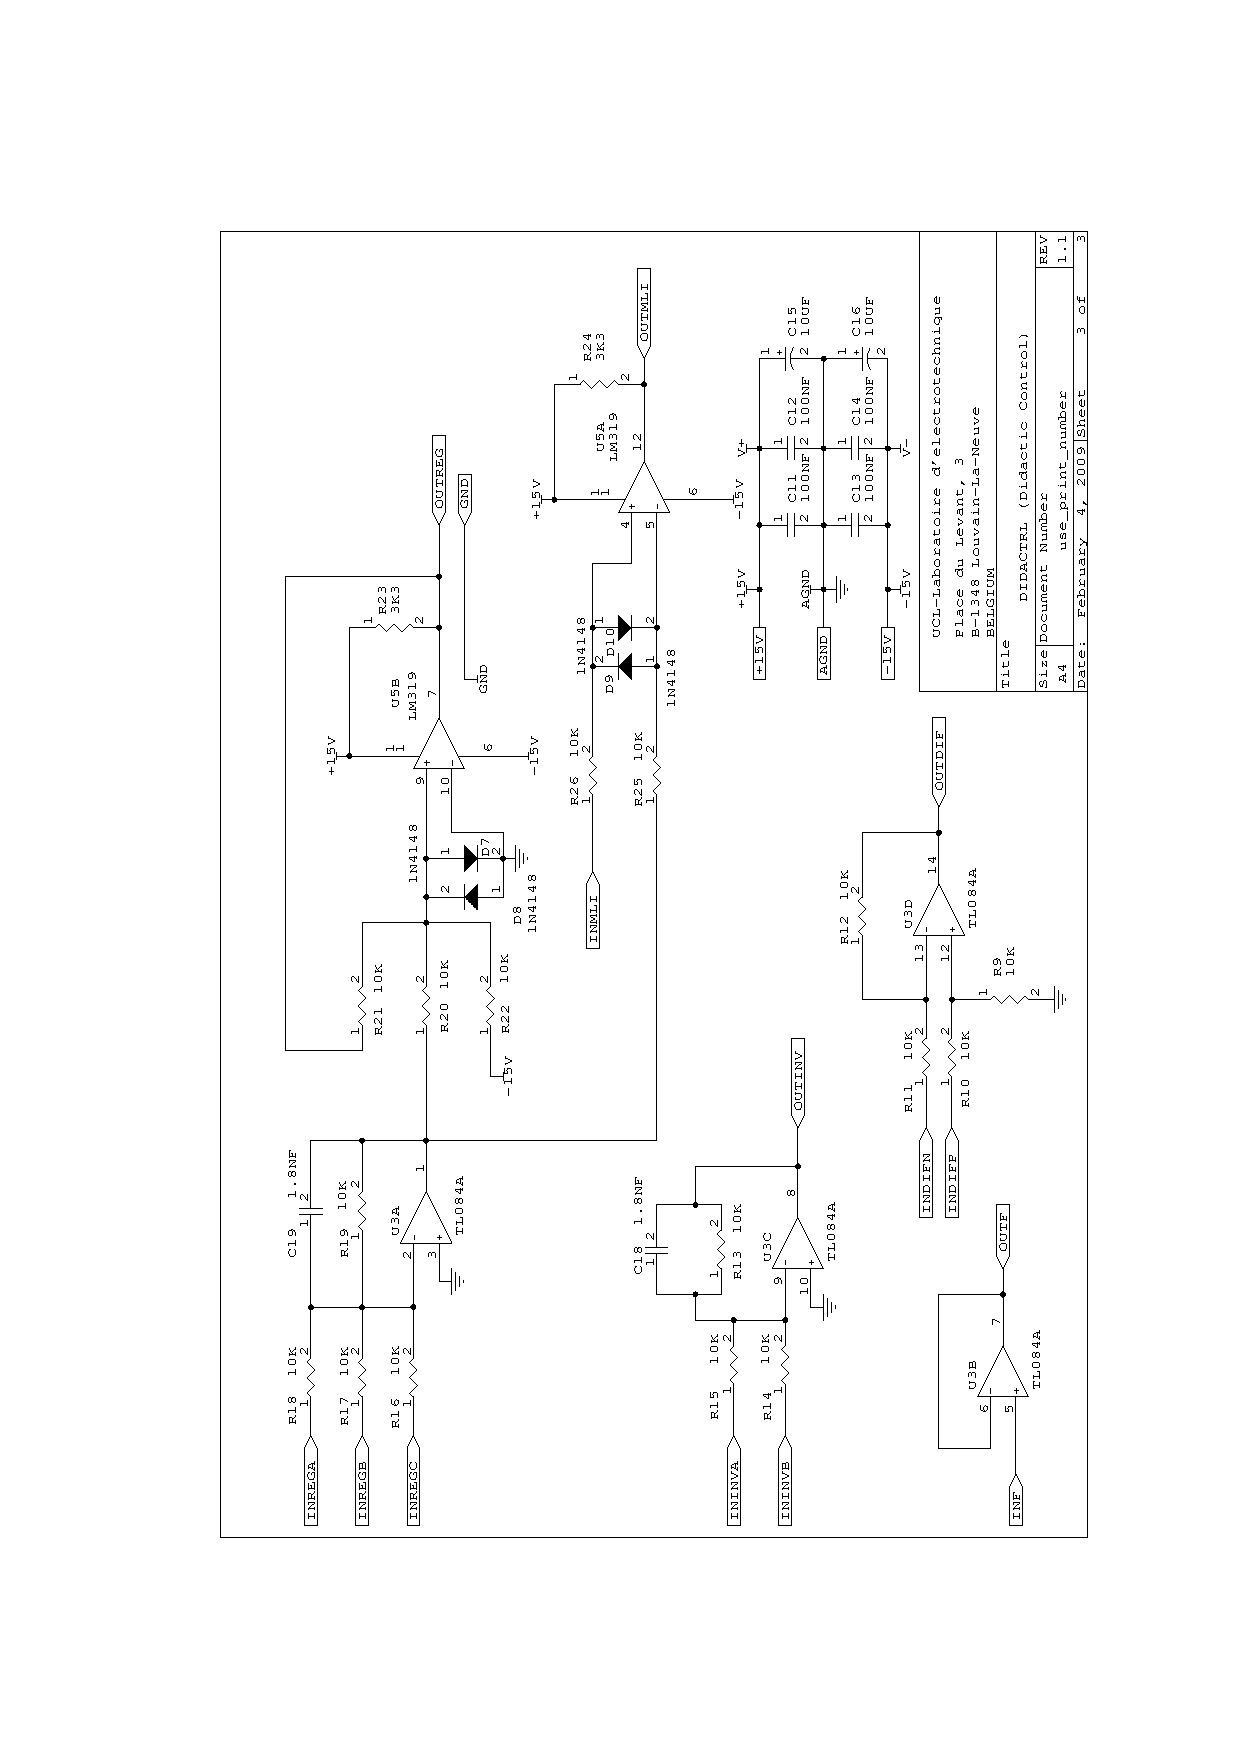
\includepdf[pagecommand=\section{Schéma du circuit DIDACTRL}]{pdf/DIDACTRL.pdf}
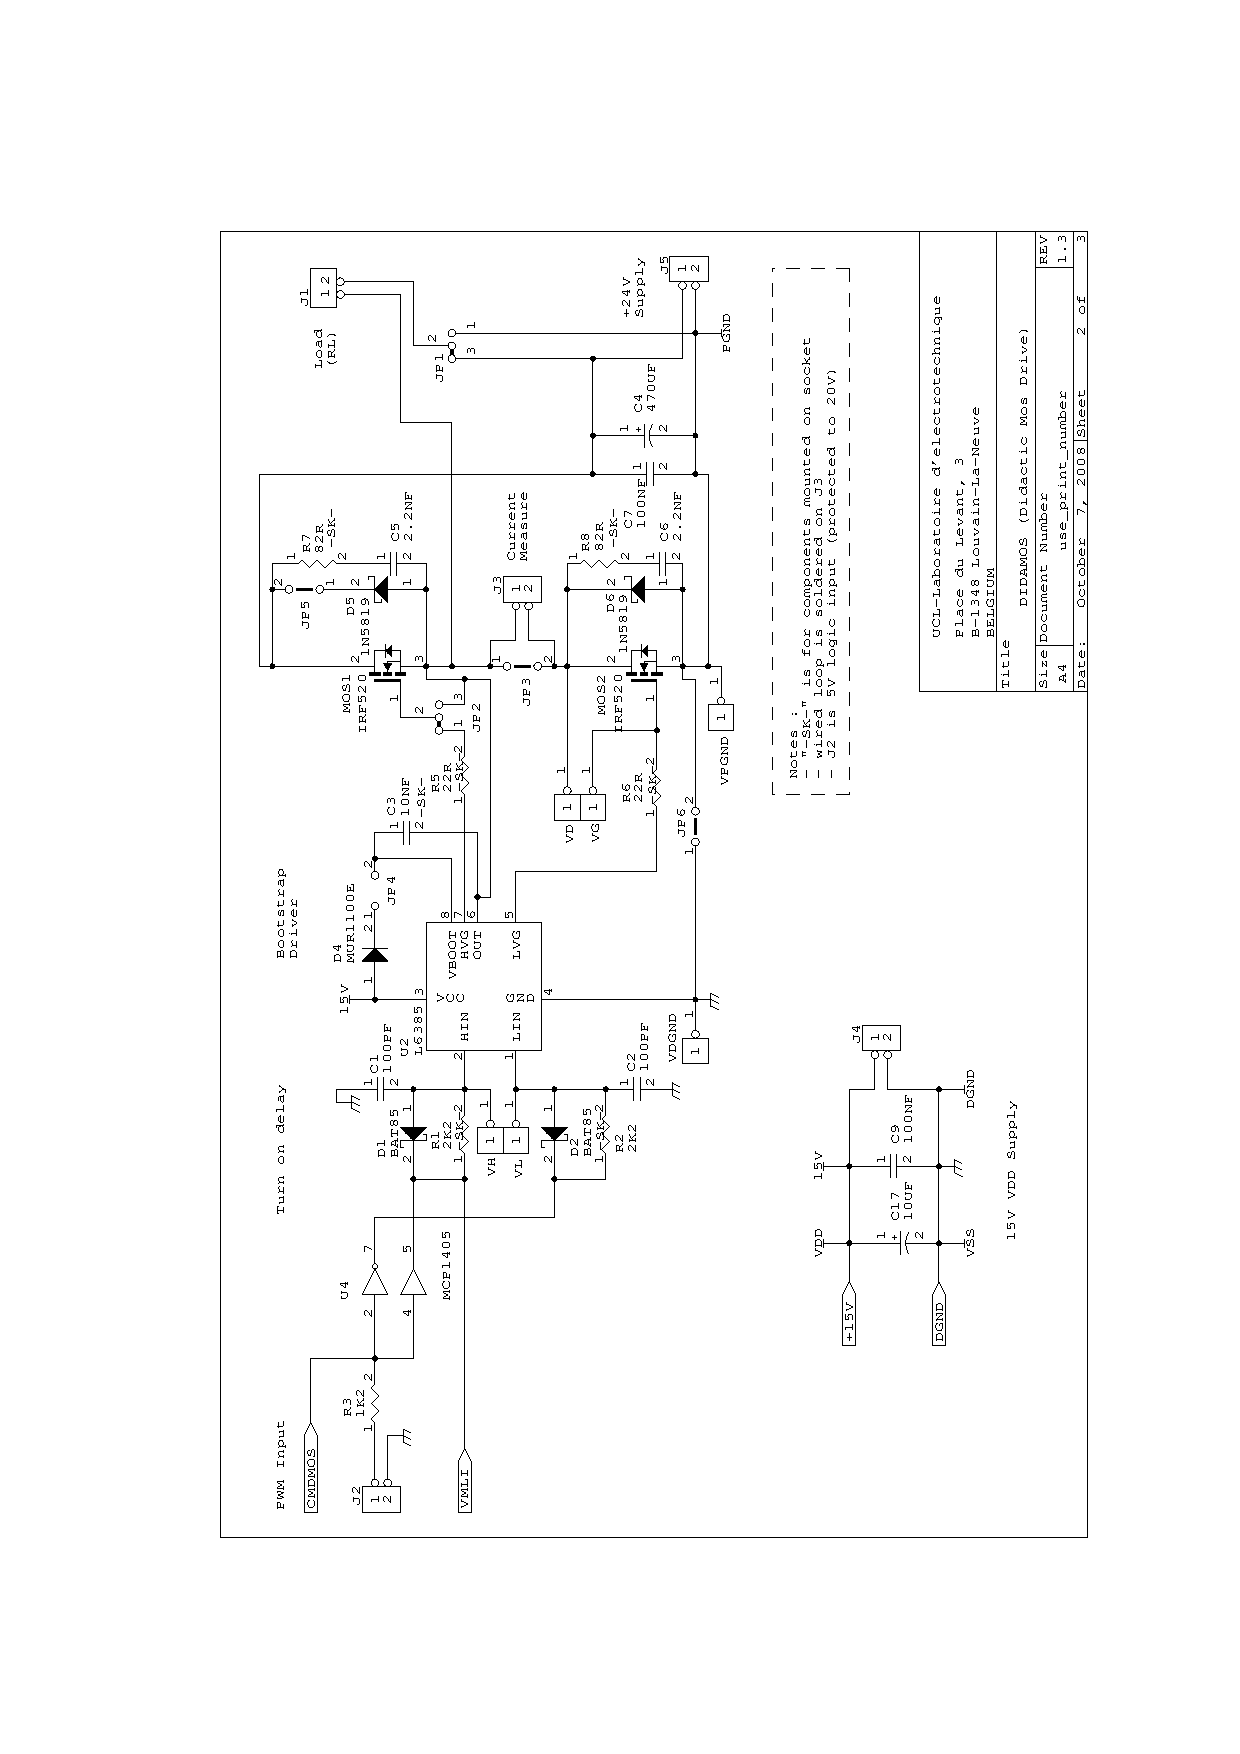
\includepdf[pagecommand=\section{Schéma du circuit DIDAMOS}]{pdf/DIDAMOS.pdf}
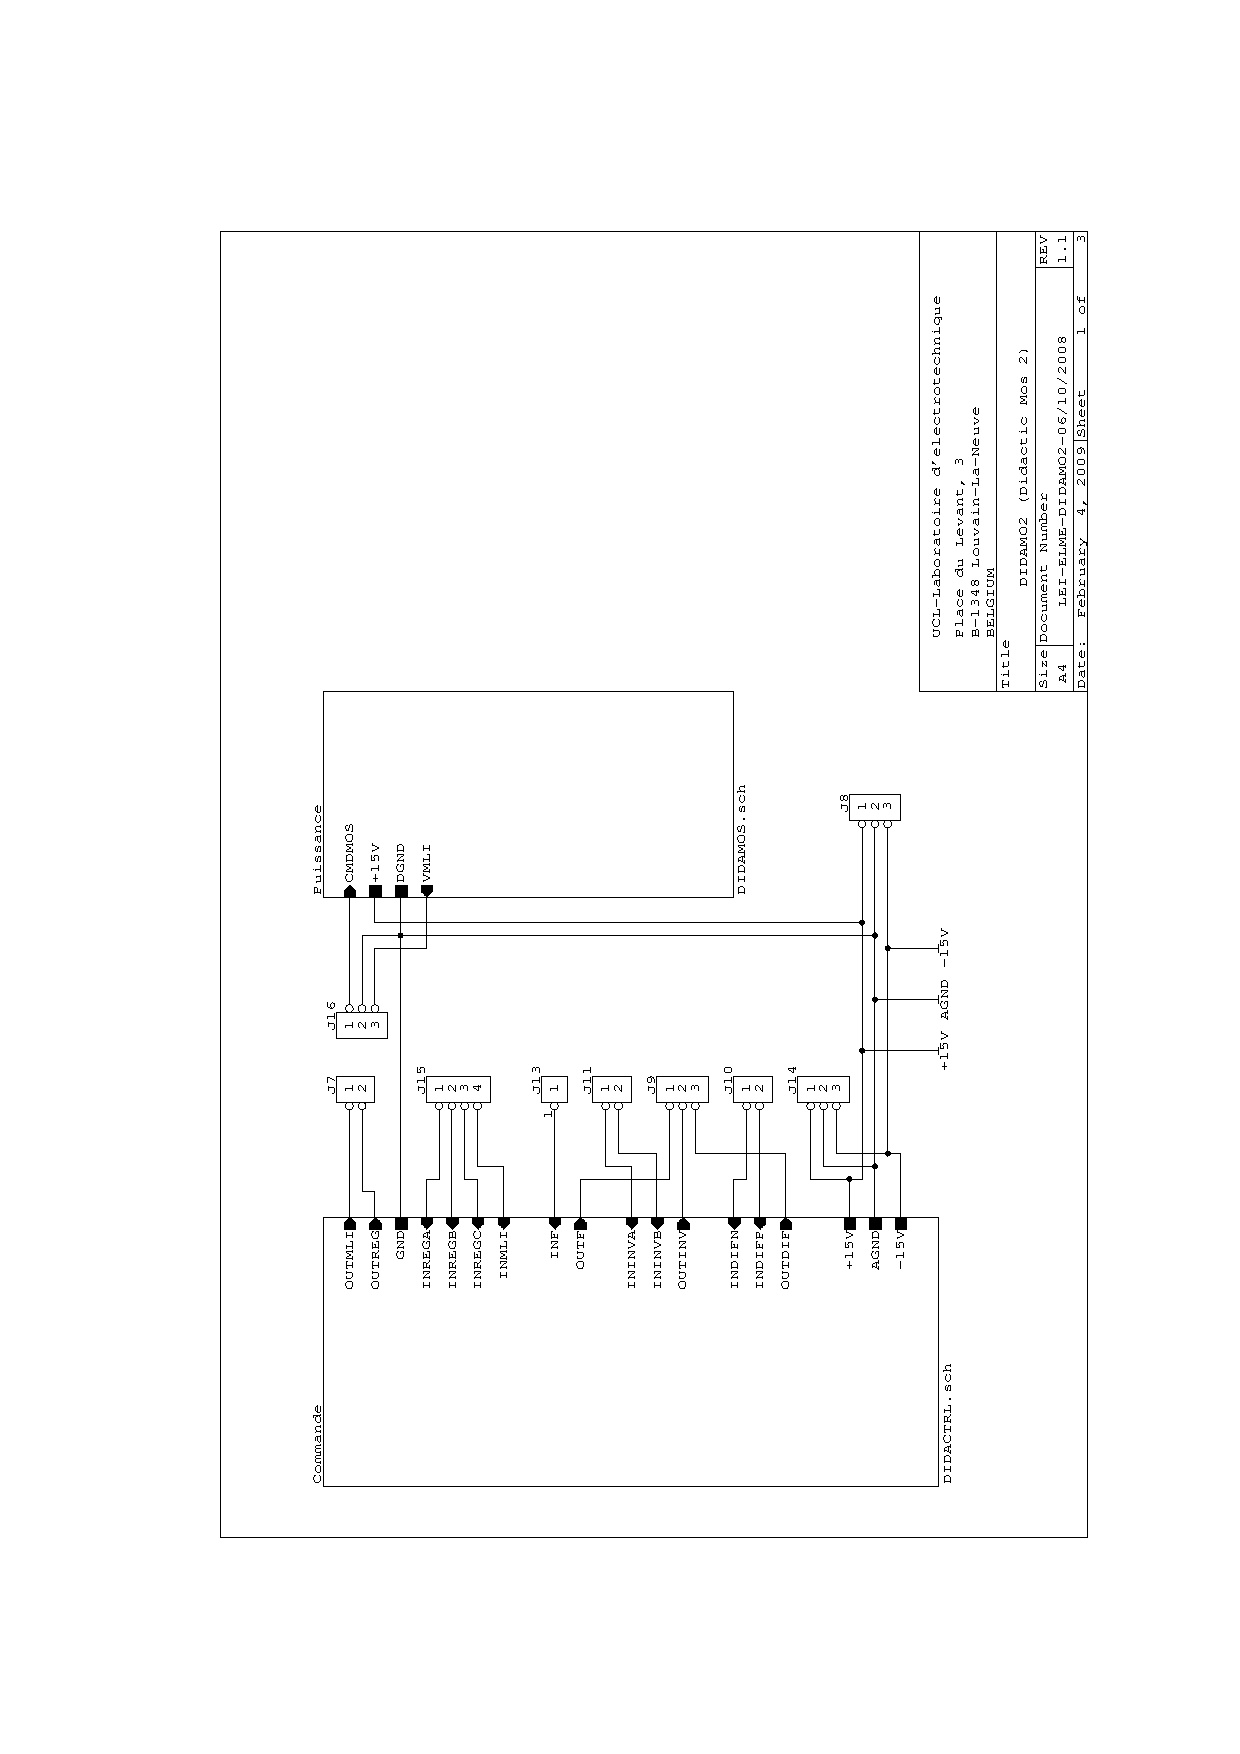
\includepdf[pagecommand=\section{Schéma du circuit DIDAMO2}]{pdf/DIDAMO2.pdf}

\end{document}
